\section{User Manual}
\label{usermanual}

\subsection{How to Install the game}
The game can be run on either an Android device, smart phone or tablet, or
the Android emulator on a computer.

Note that all screenshots are not of actual size.

In order to install the game on an Android device, follow these instructions
\begin{enumerate}
\item Copy the apk file to your Android's memory card and insert the card to
your device
\item Download and install the apk Installer from Google Play\cite{website:apk}
\item Once installed, the apk Installer will display the apk files on the
memory card
\item Click and install the bepresbingo.apk file
\item Wait for installation 
\item Launch `Bedpres Bingo' by pressing the icon in the menu
\end{enumerate}

\subsection{How to play Bedpres-Bingo}

Before the game is started on the Android application, the server must be started.

The server code can be found in the server folder in the delivered archive. The
server depends on Python, Django and Tastypie. If on a machine with Python installed,
and with Python's package manager, pip, in the path one can type the following commands
to get Django and Tastypie set up:

sudo pip install django==1.5
sudo pip install django-tastypie

Note that the `sudo' keyword is not used on Windows, only Linux and MacOSX.

After this, enter the server directory; once there issue the command:

python manage.py runserver 0.0.0.0:8000

Once this is done, you can enter the IP adress to your server on the Android App on the settings screen
to be able to connect to it. Note that the above command sets the server to run on port 8000,
and thus your app needs to connect to the same. For example: If the IP of the machine you run the server
on is 12.34.56.78, then by issuing the above command you need to enter 12.34.56.78:8000 as the hostname
in the Android application.

\subsubsection{Start new game}
In order to initiate a new game, the player will press the New Game-button.
\begin{center}
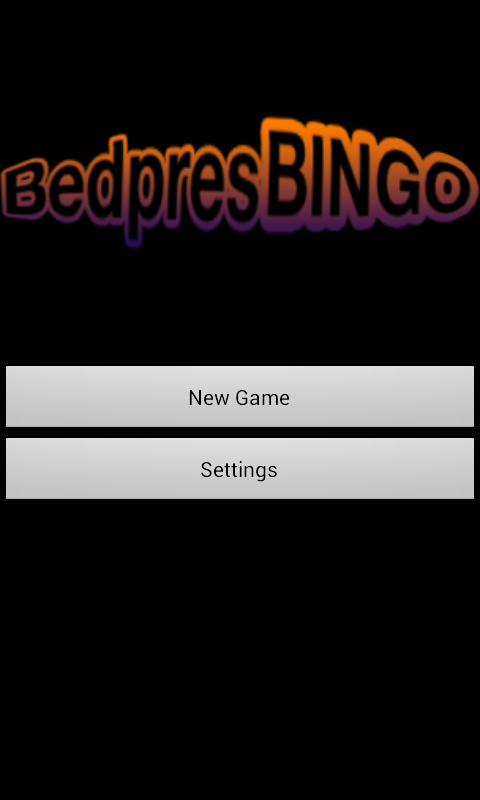
\includegraphics[scale=0.5]{Pikks/Mainmenu}
\captionof{figure}{Main menu of Bedpres Bingo}
\end{center}

Note that you will be unable to start a game unless you've set the host name of the server
as explained above, as well as set a name in the Settings. Note that the settings doesn't save
until you press the OK button (you will get a pop-up message signifying the setting has changed
if done correctly).

\subsubsection{Playing Bedres-bingo}
The main gameplay will be played on the Bingo Board shown below. The game
should be played in context of a ``Bedpres'' in order to be played properly.
The speaker will be the one presenting words. When a player hears a specific
word, the player presses the corresponding word on his/her device.

When a word is pressed, the cell with the word will turn green. The goal is to
cross off all the words in a row or column. The game is ultimately won by
crossing off all the words on the board.

\begin{center}
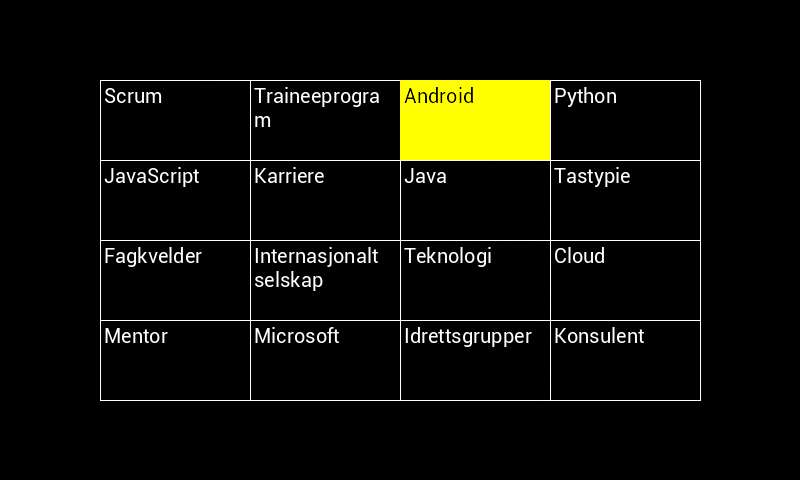
\includegraphics[scale=0.5]{Pikks/Board1}
\captionof{figure}{Main Game Screen }
\end{center}

\begin{center}
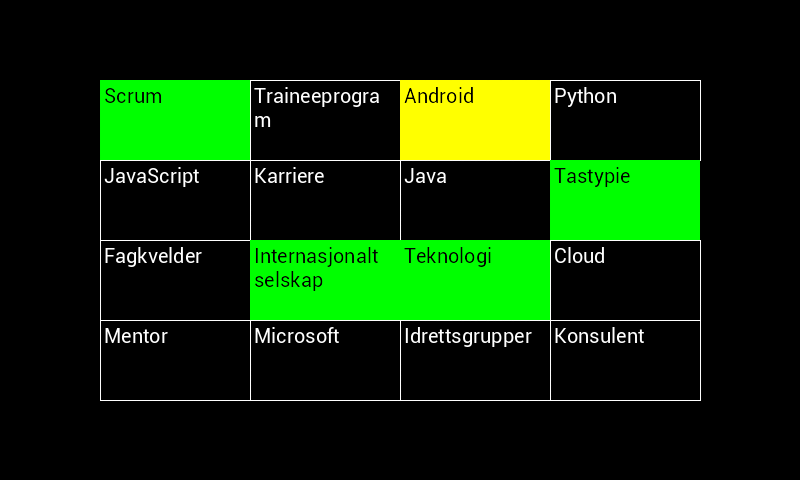
\includegraphics[scale=0.5]{Pikks/Board2}
\captionof{figure}{Board with some words selected}
\end{center}

In ``Bedpres-Bingo'', there are several goals. The name of the person
getting to each of the goals will be announced. Some of the goals have
a golden word requirement. A golden word is generated at random, placed
at a random place in random players' boards.\\\\
The goals of the ``Bedpres-Bingo'' are ranged as following:
\begin{description}
	\item[1. Golden MegaBingo]\hfill \\
		{The Golden MegaBingo is achieved if the player has a golden
		word on his/her board, and has completed the entire board.}
	\item[2. MegaBingo]\hfill \\
		{A player gets MegaBingo when he/she have completed the entire
		board.}
	\item[3. Golden TripleBingo]\hfill \\
		{The Golden TripleBingo is achieved if the player has a golden
		word on his/her board, and has completed three rows on his/her
		board.}
	\item[4. Triplebingo]\hfill \\
		{A player gets TripleBingo when he/she have completed three
		rows on his/her board.}
	\item[5. Golden DoubleBingo]\hfill \\
		{The Golden DoubleBingo is achieved if the player has a golden
		word on his/her board, and has completed two rows on his/her
		board.}
	\item[6. DoubleBingo]\hfill \\
		{A player gets DoubleBingo when he/she have completed two
		rows on his/her board.}
	\item[7. Golden SingleBingo]\hfill \\
		{The Golden SingleBingo is achieved if the player has a golden
		word on his/her board, and has completed one row on his/her
		board.}
	\item[8. SingleBingo]\hfill \\
		{A player gets SingleBingo when he/she have completed one
		row on his/her board.}
\end{description}


\subsubsection{Change your name}
In accordance with FR2: ``Set player names'', the players should be able to
change their name. This is done via the settings menu. The player may enter a
name, and press the OK-button in order to change the name that will be used
in-game.

\begin{center}
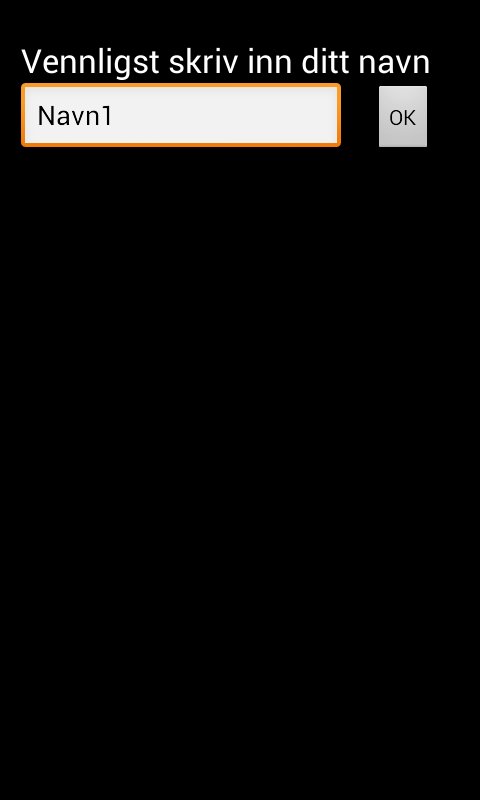
\includegraphics[scale=0.5]{Pikks/Settings1}
\captionof{figure}{Settings screen}
\end{center}

\subsection{Reconnecting to the ongoing game}
In some cases the player could encounter the need to reconnect to the
ongoing game, wether the reasons are loss of internet connection,
or exiting the application. To reconnect, the user should simply
navigate to the main menu of the app, and press the ``Join Game''
button. The player will then be able to continue playing the 
``Bedpres-Bingo'' he or she joined at the beginning of the ``Bedpres''.


\subsection{Scoring points and winning}
When a player crosses off all words in a vertical/horizontal/diagonal line, the player has achieved a bingo. If another player is the first player to get bingo of a specific kind, the other players are notified that someone was first to achieve bingo. This is shown in the figures below.

\begin{center}
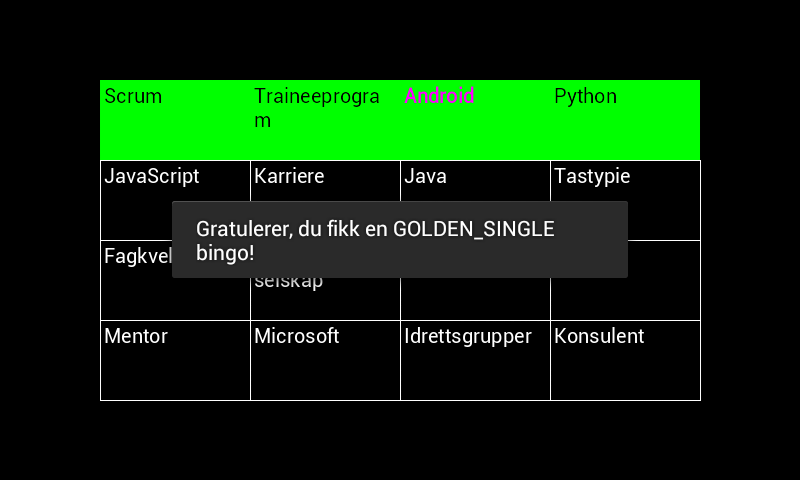
\includegraphics[scale=0.5]{Pikks/GoldenSingle}
\captionof{figure}{You achieved a Golden Single Bingo}
\end{center}

\begin{center}
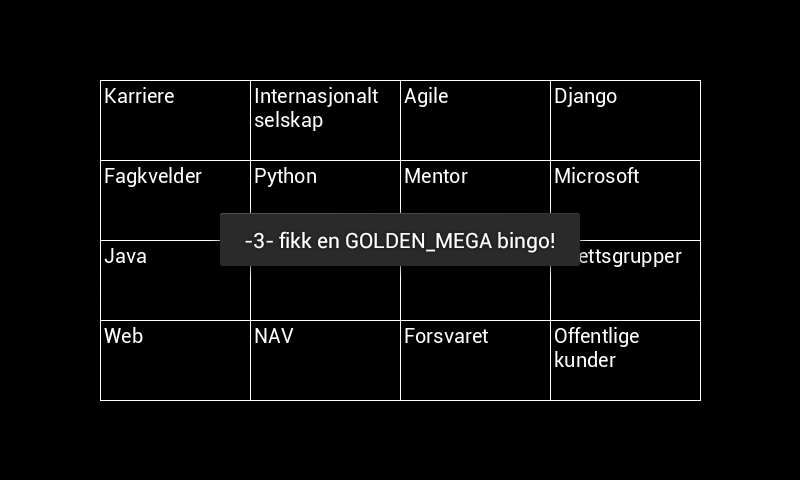
\includegraphics[scale=0.5]{Pikks/Notificationfromserver}
\captionof{figure}{Another player achieved bingo first}
\end{center}


The game is ultimately won by achieving a MEGA-Bingo or a Golden MEGA-BINGO. 

\begin{center}
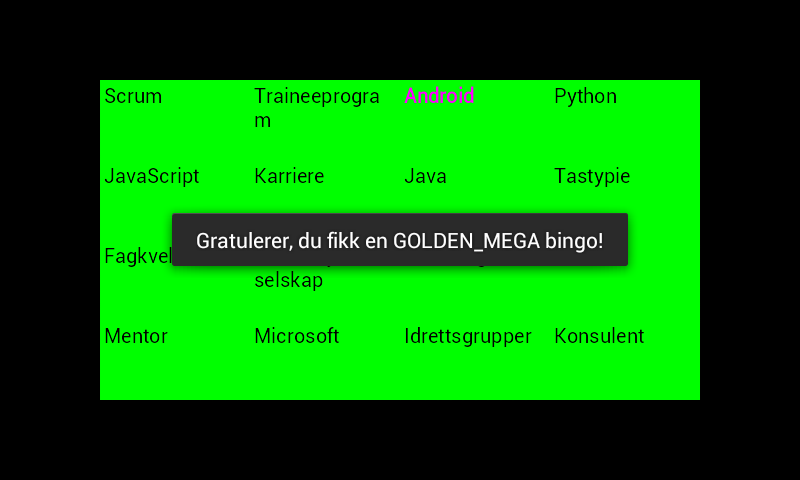
\includegraphics[scale=0.5]{Pikks/GoldenMega}
\captionof{figure}{You achieved a Golden Mega-Bingo. Congratulations!}
\end{center}
